\part{Recherche Opérationnel}
\pagebreak

\chapter{Rappel}
\section{Pivot de gauss}

$ L1 et L2 =
\begin{cases}
L1: 160 = 8x + 4y\\
L2: 120 = 4x + 6y 
\end{cases}$
\\
$( L2*(-2) )=
\begin{cases}
L1: 160 = 8x + 4y\\
L2: -240 = -8x -12y
\end{cases}$
\\
$( L2=L2+L1 )=
\begin{cases}
L1: 160 = 8x + 4y\\
L2: -80 = -8y
\end{cases}$
\\
$y = 10$
\\\\
$8x + 4*10 = 160$\\
$8x + 40 = 160$\\
$8x = 120$\\
$x = 15$\\

\chapter{Introduction à la PL}

Construire une modèle linéaire, c'est donc:
\begin{description}
\item[identifier] les variables de décision du problème
\item[déterminer]: la fonction objectif du modèle
\item[déterminer]: les contraintes du modèle 
\end{description}

\section{Modèle linéaire continus à 2 variables}
Soit le modèle linéaire suivantes:
\begin{description}
\item[Déterminer] $(x,y) \in \Im^2$
\item[Minimisant] $z = 1000x + 1200y$
\item[sous les contraintes]:
\begin{description}
\item[] $(1) 8x + 4y \leq 160$
\item[] $(2) 4x + 6y \leq 120$
\item[] $(3) x \leq 34$
\item[] $(4) y \leq 14$
\item[] $(5) 0 \leq x$
\item[] $(6) 0 \leq y$
\end{description}
\end{description}

\subsection{Recherche de solutions}
Après avoir tracé graphiquement tout les points:\\
Pour chaque contrainte, tracer la droite et repérer le demi plan des solution: exemple pour (5) et (6), x et y doivent être supérieurs ou égal à 0, d'où le demi plan des solution sont toutes les valeurs positives.\\
La partie En vert représente la région admissible, quelque soit le point choisis dans ce vert, aucune contrainte ne sera violé.\\
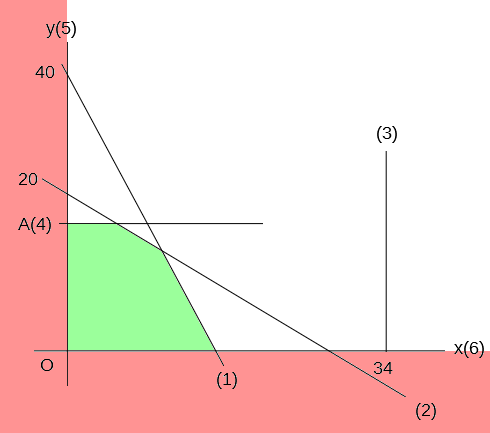
\includegraphics[scale=0.55]{img/ro-pl-2var_0.png} 
\subsection{recherche de la solution optimal}

Changer l'équation $z$ tel que $z$ soit égal à $0$
\begin{description}
\item[$z$] = $1000x + 1200y$ = $0$ = $1000*(1200) + 1200 *(-1000)$
\end{description}
Traçons la droite $(0,0)$, $(1200,-1000)$
\begin{description}
\item[Un point extrême]: est un point se trouvant sur l'intersection de 2 contraintes et étant dans la zone admissible.
\item[L'altitude]: est la droite (rouge) la plus haute touchant un point extrême, ce point sera le vecteur $(x,y)$ le plus optimal pour $z$.
\item[] Les droites rouges doivent être toutes parallèles.
\end{description}
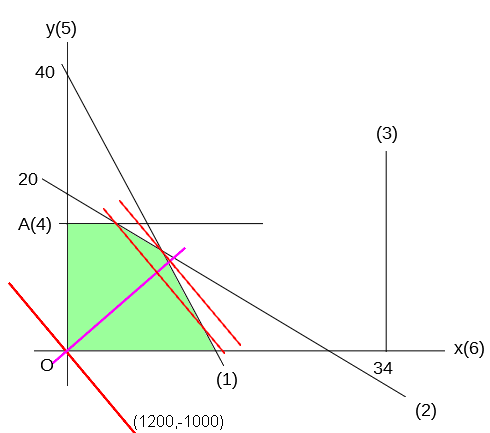
\includegraphics[scale=0.55]{img/ro-pl-2var_1.png} \\
Dans cette exemple le point (15,10) est le point extrême maximal pour l'équation z.\\
\pagebreak
\chapter{Le simplexe}
Soit le modèle linéaire suivantes:
\begin{description}
\item[Déterminer] $(x,y) \in \Im^2$
\item[Maximisant] $Z = 3x + 7y$
\item[sous les contraintes]:
\begin{description}
\item[] (1) $ -x + y \leq 3$
\item[] (2) $ y \leq 8$
\item[] (3) $ 2x - y \leq 28$
\item[] (5) $ 0 \leq x$
\item[] (6) $ 0 \leq y$
\end{description}
\end{description}

\section{Initialisation du simplexe}
Pour chaque expression du type $(1)(2)(3)$ intégrer un $e_i$ pour la transformer en équation.\\
On appel les $e_1$ des variables d'accumulation, Ce qui fait\\
\begin{description}
\item[Déterminer] $(x,y,e_1,e_2,e_3) \in \Im^5$
\item[Maximisant] $Z = 3x + 7y$
\item[sous les contraintes]:
\begin{description}
\item[] (1) $ -x + y + e_1 = 3$
\item[] (2) $ y + e_2 = 8$
\item[] (3) $ 2x - y + e_3 = 28$
\item[] (5) $ 0 \leq x$
\item[] (6) $ 0 \leq y$
\item[] (7) $ e_1,e_2,e_3 \geq 0$
\end{description}
\end{description}

\section{Canonicité du modèle}
Soit les valeurs (pour la première itération)
\begin{description}
\item[Hors Base] $(x,y)$
\item[Base] $(e_1,e_2,e_3)$
\end{description}

Un modèle est canonique que si:
\begin{description}
\item[si toutes les variables de Base] ne sont pas dans Z.
\end{description}

\section{Solution admissible}
\begin{description}
\item[] (1) $-x + y + e_1 = 3$
\item[] (2) $x - e_1 + e_2 = 5$
\item[] (3) $3x - e_1 + e_3 = 25$
\item[Variable hors base] = $x,e_1$
\item[Variable Base] = $y,e_2,e_3$
\item[Avec comme solution admissible] $A\ Deduire (x,y,e_1,e_2,e_3)$
\end{description}
\ \\
Pour toute variable présente dans l'ensemble $Hors\ base$ la valeur admissible est égal à $0$\\
Donc solution admissible = $(0, y, 0, e_2, e_3)$\\
Les 3 dernières valeurs sont les résultat des équations (soit $3$, $5$ et $25$).\\
Pour chaque équation nous lisons les termes de droit à gauche et ignorons ceux qui sont dans l'ensemble $Hors\ Base$:\\
Donc solution admissible = $(0, 3, 0, 5, 25)$\\

\section{Exemple simple Premier itération}
\subsection{Choix de la variable entrante}
\begin{description}
\item[Gain marginale] prendre la variable non négatif ayant le plus haut coefficient.
\end{description}
$(x,y)$ sont deux choix possible, le tout est de choisir une bonne heuristique, comme celle du meilleur gain marginale, ou via la comparaison (en mode graphique):\\
$Y$ sera choisit, donc $Y$ sera notre variable entrante.\\

\subsection{Choix de la variable sortante}
Pour chaque résultat d'équation, le diviser par sa valeur de $Y$ (le résultat devant être positif sinon l'ignorer)\\

\begin{description}
\item[] $ -x + y + e_1 = 3$ donne $\frac{3}{\crouge{1}} = 3$ (1 car $y$ = $1*y$)
\item[] $ y + e_2 = 8$ donne $\frac{8}{1} = 8$
\item[] $ 2x - y + e_3 = 28$ donne $\frac{28}{1} = 28$
\end{description}
Prendre le minimum des variables, donc se sera $3$.\\
la variable présente dans la Base sera prise comme variable sortante, dans notre cas $e_1$.\\
\pagebreak
\subsection{pivotage}
On choisis l'équation associé à la variable $e_1$ pour définir la variable entrante $y$.\\
On n'a:
\begin{description}
\item[$y$] = $\frac{1}{\crouge{1}}*(x - e_1 + 3)$
\end{description}

Puis on crée les nouvelles équations via le nouveau $y$:
\begin{description}
\item[$Z = 3x + 7y$] devient
\begin{description}
\item[$Z$] = $3x + 7(x - e_1 + 3)$
\item[$Z$] = $10x - 7e_1 + 27$
\end{description}
\item[$x - e_1 = 3$] est déjà normalisé
\item[$y + e_2 = 8$] devient
\begin{description}
\item[$8$] = $x -e_1 + 3 + e_2$
\item[$5$] = $x - e_1 + e_2$
\end{description}
\item[$2x - y + e_3 = 28$] devient
\begin{description}
\item[$28$] = $2x + (x - e_1 + 3) + e_3$
\item[$25$] = $3x - e_1 + e_3$
\end{description}
\end{description}
\subsection{Nouveau modèle}
\romodel{$(x,y,e_1,e_2,e_3) \in \Im^5$}
        {Maximisant}{$Z = 10x - 7e_1 + 21$}
        {$x,e_1$}{$y,e_2,e_3$}{$(0,3,0,5,25)$}{$21$}
        {\begin{description}
\item[] (1) $-x + y + e_1 = 3$
\item[] (2) $x - e_1 + e_2 = 5$
\item[] (3) $3x - e_1 + e_3 = 25$
\item[] (5) $ 0 \leq x$
\item[] (6) $ 0 \leq y$
\item[] (7) $ e_1,e_2,e_3 \geq 0$
\end{description}
}

A ne pas oublier de vérifier la canonicité du modèle.\\

\section{Exemple simple Seconde itération}
\subsection{Choix de la variable entrante}
$X$ sera choisit, donc $X$ sera notre variable entrante.\\

\subsection{Choix de la variable sortante}
\begin{description}
\item[] $\frac{5}{\crouge{1}} = 5$
\item[] $\frac{25}{3} = 8.3$
\end{description}
Prendre le minimum des variables, donc se sera $5$, donc $e_2$.\\

\subsection{pivotage}
\begin{description}
\item[$x$] = $\frac{1}{\crouge{1}}*(e_1 - e_2 + 5)$
\end{description}

Puis on crée les nouvelles équations via le nouveau $y$:
\begin{description}
\item[$Z = 10x - 7e_1 + 27$] devient
\begin{description}
\item[$Z$] = $10(e_1 - e_2 + 5) - 7e_1 + 27$
\item[$Z$] = $3e_1 - 10e_2 + 71$
\end{description}
\item[$-x + y + e_1 = 3$] devient
\begin{description}
\item[$3$] = $-(e_1 - e_2 + 5) + y + e_1$
\item[$8$] = $y + e_2$
\end{description}
\item[$3x - e_1 + e_3 = 25$] devient
\begin{description}
\item[$25$] = $3(e_1 - e_2 + 5) -e_1 + e_3$
\item[$10$] = $2e_1 - 3e_2 + e_3$
\end{description}
\end{description}

\subsection{Nouveau modèle}
\romodel{$(x,y,e_1,e_2,e_3) \in \Im^5$}
        {Maximisant}{$Z = 3e_1 - 10x + 71$}
        {$e_2,e_1$}{$y,x,e_3$}{$(5,8,0,0,10)$}{$71$}
        {\begin{description}
\item[] (1) $y + e_2 = 8$
\item[] (2) $x - e_1 + e_2 = 5$
\item[] (3) $2e_1 - 3e_2 + e_3 = 10$
\item[] (5) $ 0 \leq x$
\item[] (6) $ 0 \leq y$
\item[] (7) $ e_1,e_2,e_3 \geq 0$
\end{description}
}

A ne pas oublier de vérifier la canonicité du modèle.\\

\section{Exemple simple, troisième itération}
\subsection{Variable entrante et sortante}
\rovarinout{$e_1$}{$e_3$}
  {$\frac{8}{0}$ est NULL}
  {$\frac{5}{1}$ car négatif}
  {$\frac{10}{2} = 5$}

\subsection{Nouveau modèle}
\romodel{$(x,y,e_1,e_2,e_3) \in \Im^5$}
        {Maximisant}{$Z = 86 - \frac{11}{2}e_2 - \frac{3e_3}{2}$}
        {$e_2,e_3$}{$y,x,e_1$}{$(10,8,5,0,0)$}{$86$}
        {\begin{description}
\item[] (1) $- \frac{1}{2}e_2 + \frac{e_3}{2} + e1 = 10$
\item[] (2) $e_2 + y = 8$
\item[] (3) $e_1 - \frac{3}{2}e_2 + \frac{e_3}{2} = 5$
\item[] (5) $ 0 \leq x$
\item[] (6) $ 0 \leq y$
\item[] (7) $ e_1,e_2,e_3 \geq 0$
\end{description}
}
\section{Exemple simple, dernière itération}
Stop car $e_2$ et $e_3$ sont inférieur à 0 dans $Z$.

\chapter{Simplexe à deux phases}
Soit le modèle suivant:
\begin{description}
\item[Déterminer] $(x,y) \in \Im^2$
\item[Maximisant] $Z = 2x + 3y$
\item[sous les contraintes]:
\begin{description}
\item[] (1) $x + y \leqslant 4$
\item[] (2) $x + 2y \leqslant 5$
\item[] (3) $4x -y \geqslant 2$
\item[] (4-5) $x,y \geqslant 0$
\end{description}
\end{description}

Lorsque le sens de l'équation est $\leqslant$ il faut ajouter une variable $e_i$, dans le cas des équations $\geqslant$
il faut ajouter une variable d'excédant $a$ dans la contrainte concerné et instaurer $Z$ à $- a$\\
La représentation graphique ci dessous:\\
\begin{center}
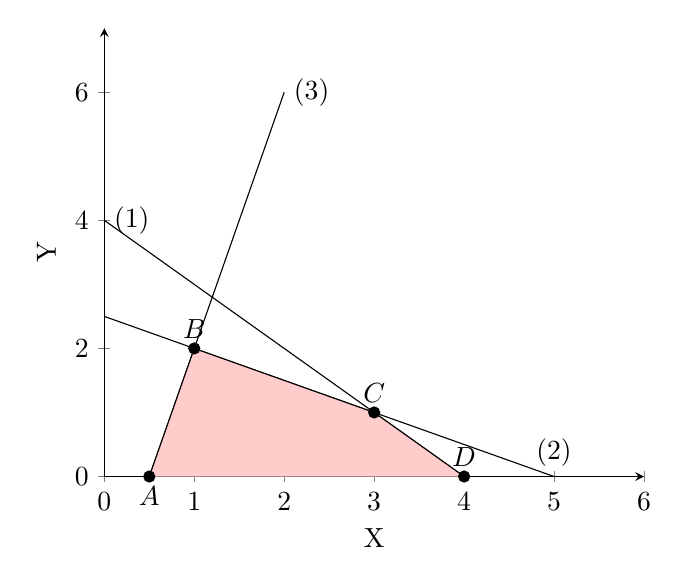
\begin{tikzpicture}
  \begin{axis} [
      xlabel     = X, % label x axis
      ylabel     = Y, % label y axis
      axis lines = left, %set the position of the axes
      clip       = false, 
      xmin       = 0,
      ymin       = 0,
      xmax       = 6,
      ymax       = 7,
    ]
    \addplot [color=black] coordinates { (4,0)(0,4) } node[right] {$(1)$};
    \addplot [color=black] coordinates { (0,2.5)(5,0) } node[above] {$(2)$};
    \addplot [color=black] coordinates { (0.5,0)(2,6) } node[right] {$(3)$};
    
    \addplot [only marks, mark=*, color=black] coordinates { (0.5,0) } node[below] {$A$};
    \addplot [only marks, mark=*, color=black] coordinates { (1,2) } node[above] {$B$};
    \addplot [only marks, mark=*, color=black] coordinates { (3,1) } node[above] {$C$};
    \addplot [only marks, mark=*, color=black] coordinates { (4,0) } node[above] {$D$};
    
    \addplot [color=black, style={fill=red!20}] coordinates { (0.5,0)(1,2)(3,1)(4,0) };
  \end{axis}
\end{tikzpicture}
\end{center}
\section{Première phase du simplexe à deux phases}
Pour toutes expression sous la forme $ A \geqslant -i$, multiplier les deux coté par $-1$ et inverser le signe pour obtenir des équations positif.\\
Si une contrainte est jugé redondante, alors elle peut être éliminé sans changer le modèle.\\
Le modèle ci dessus n'est pas canonique, donc nous allons exprimer $Z$ en fonction de l'équation portant le symbole $a$:\\
\subsection{Nouveau modèle}
\romodel{$(x,y,e_1,e_2,e_3,a) \in \Im^5$}
        {Maximisant}{$Z = -a = 4x -y -e_3 -2\ \ \cgris{\% oldZ = 2x + 3y}$}
        {$x,y,a$}{$e_1,e_2,e_3$}{$(0,0,4,5,0,2)$}{$-2$}
        {\begin{description}
\item[] (1) $x + y + e_1 = 4$
\item[] (2) $x + 2y + e_2 = 5$
\item[] (3) $4x -y - e_3 + a = 2$
\item[] (4-5) $x,y,e_i,a \geqslant 0$
\end{description}
}
Ce modèle est canonique.

\section{Premier phase du simplexe à deux phases, première itération}
\subsection{Variable entrante et sortante}
\rovarinout{$x$}{$a$}
  {$\frac{4}{1}$}
  {$\frac{5}{1}$}
  {$\frac{2}{4} = \crouge{\frac{1}{2}}$}

\subsection{pivotage}
\begin{description}
\item[$x$] = $\crouge{\frac{1}{2}}*(y+ e_3 -a +2) = \frac{y}{4} + \frac{e_3}{4} - \frac{a}{4} + \frac{1}{2}$
\end{description}

\subsection{Nouveau modèle}
\romodel{$(x,y,e_1,e_2,e_3,a) \in \Im^5$}
        {Maximisant}{$Z = -a \\ \cgris{\% oldZ = 2x + 3y}$}
        {$y,a$}{$e_1,e_2,x$}{$(\frac{1}{2},0,\frac{7}{2}, \frac{9}{2}, 0,0)$}{$0$}
        {\begin{description}
\item[] (1) $\frac{5}{4}y + e_1 + \frac{e_3}{4} - \frac{a}{4} = \frac{7}{2}$
\item[] (2) $\frac{9}{4}y + e_2 + \frac{e_3}{4} - \frac{a}{4} = \frac{9}{2}$
\item[] (3) $x - \frac{y}{4} - \frac{e_3}{4} + \frac{a}{4} = \frac{1}{2}$
\item[] (4-5) $x,y,e_i,a \geqslant 0$
\end{description}
}

\section{Premier phase du simplexe à deux phases, seconde itération}
Nous somme en présente d'un système optimal car $Z$ à l'altitude 0.\\
Une solution admissible serait $(PG=)$:
\begin{description}
\item[$A(\frac{1}{2},0)$] est le point extrême correspondant:
\item[] \begin{description}
\item[] $y_A = 0$
\item[] $4x_A - y_A = 2$
\end{description}
\end{description}

Comme $z = 0$ on passe en phase 2.
\section{Seconde phase du simplexe à deux phases}
\romodel{$(x,y,e_1,e_2,e_3) \in \Im^5$}
        {Maximisant}{$Z = oldZ = 2x + 3y$}
        {$y$}{$e_1,e_2,x$}{$(\frac{1}{2},0,\frac{7}{2}, \frac{9}{2}, 0)$}{$0$}
        {\begin{description}
\item[] (1) $\frac{5}{4}y + e_1 + \frac{e_3}{4} = \frac{7}{2}$
\item[] (2) $\frac{9}{4}y + e_2 + \frac{e_3}{4} = \frac{9}{2}$
\item[] (3) $x - \frac{y}{4} - \frac{e_3}{4} = \frac{1}{2}$
\item[] (4-5) $x,y,e_i \geqslant 0$
\end{description}
}\ \\
On retire toutes les occurrences de $a$.\\
Le modèle n'est pas canonique car $x$ est hors base, donc remplacer $x$ dans $Z$ car il est définit:\\
$Z = 2x + 3y = 2(\frac{y}{4} + \frac{e_3}{4} + \frac{1}{2}) + 3y = \frac{7}{2}y + \frac{e_3}{2} + 1$\\

\romodel{$(x,y,e_1,e_2,e_3) \in \Im^5$}
        {Maximisant}{$Z = \frac{7}{2}y + \frac{e_3}{2} + 1$}
        {$y,e_3$}{$e_1,e_2,x$}{$(\frac{1}{2},0,\frac{7}{2}, \frac{9}{2}, 0)$}{$1$}
        {\begin{description}
\item[] (1) $\frac{5}{4}y + e_1 + \frac{e_3}{4} = \frac{7}{2}$
\item[] (2) $\frac{9}{4}y + e_2 + \frac{e_3}{4} = \frac{9}{2}$
\item[] (3) $x - \frac{y}{4} - \frac{e_3}{4} = \frac{1}{2}$
\item[] (4-5) $x,y,e_i \geqslant 0$
\end{description}
}
Ce modèle est canonique.

\section{Seconde phase du simplexe à deux phases, première itération}
\subsection{Variable entrante et sortante}
\rovarinout{$y$}{$e_2$}
  {$\frac{\frac{7}{2}}{\frac{5}{4}} = \frac{14}{5}$}
  {$\frac{\frac{9}{2}}{\crouge{\frac{9}{4}}} = 2$}
  {$ \leqslant 0 $}

\subsection{pivotage}
\begin{description}
\item[$y$] = $\crouge{\frac{4}{9}}*(- e_2 - \frac{e_3}{4} + \frac{9}{2}) = - \frac{4}{9} e_2 - \frac{e_3}{9} + 2$
\end{description}

\subsection{Nouveau modèle}
\romodel{$(x,y,e_1,e_2,e_3) \in \Im^5$}
        {Maximisant}{$Z = -\frac{14}{9}e_2 + \frac{e_3}{9} + 8$}
        {$e_2,e_3$}{$e_1,y,x$}{$(1,2,1,0,0)$}{$8$}
        {\begin{description}
\item[] (1) $x - \frac{5}{9} e_2 + \frac{e_3}{9} = 1$
\item[] (2) $y + \frac{4}{9} e_2 + \frac{e_3}{9} = 2$
\item[] (3) $x + \frac{e_2}{9} - \frac{2}{9}e_3 = 1$
\item[] (4-5) $x,y,e_i \geqslant 0$
\end{description}
}
Ce modèle est canonique.

\section{Seconde phase du simplexe à deux phases, seconde itération}
\subsection{Variable entrante et sortante}
\rovarinout{$e_3$}{$e_1$}
  {$\frac{1}{\frac{1}{9}} = \crouge{9}$}
  {$\frac{2}{\frac{1}{9}} = 18$}
  {$ \leqslant 0$}
  
\subsection{pivotage}
\begin{description}
\item[$e_3$] = $9(-e_1 + \frac{5}{9}e_2 + 1) = -9e_1 + 5e_2 + 9$
\end{description}

\subsection{Nouveau modèle}
\romodel{$(x,y,e_1,e_2,e_3) \in \Im^5$}
        {Maximisant}{$Z = -e_1 -e_2 + 9$}
        {$e_2,e_1$}{$e_3,y,x$}{$(3,1,0,0,9)$}{$9$}
        {\begin{description}
\item[] (1) $9y + 5e_2 + e_3 = 9$
\item[] (2) $y - e_1 + e_2 = 1$
\item[] (3) $x + 2e_1 - e_2 = 3$
\item[] (4-5) $x,y,e_i \geqslant 0$
\end{description}
}
Ce modèle est canonique.

\section{Seconde phase du simplexe à deux phases, troisième itération}
Il n'existe pas de variable entrante car $e_1$ et $e_3 \leqslant 0$
\pagebreak